\documentclass[12pt]{article}
\usepackage{graphicx} %required for inserting images
\graphicspath{{./images/}}
\usepackage{array}
\usepackage{lipsum}
\usepackage{comment}
\usepackage{amsmath}
\usepackage{wrapfig}
%flowchart drawing package




%Tiles making sections
\title{GEOTECHNICAL DESIGN OF RAMMED AGGREGATE COLUMN}
\author{Sakib Bin Rafi Tonmoy,Jakaria Pervez}
\date{27/04/2023}
%End for tiltles
\begin{document}
\maketitle

%%Begining of Introduction
\section{Installtion Process for Rammed Aggregate Column }
 Rammed Aggregate column  can be install without using any specilized equipments.Indeginous method for Boring and Using of 1500kg to 2000kg rammer shall be sufficient for this type of column.Cost shall be 1/3 of RCC piles.Usually finished pile diameter is 1.5-2 times the casing dia.
  \\


%%adding figure for rammed aggregate instllation
\begin{figure}[h]
\centering
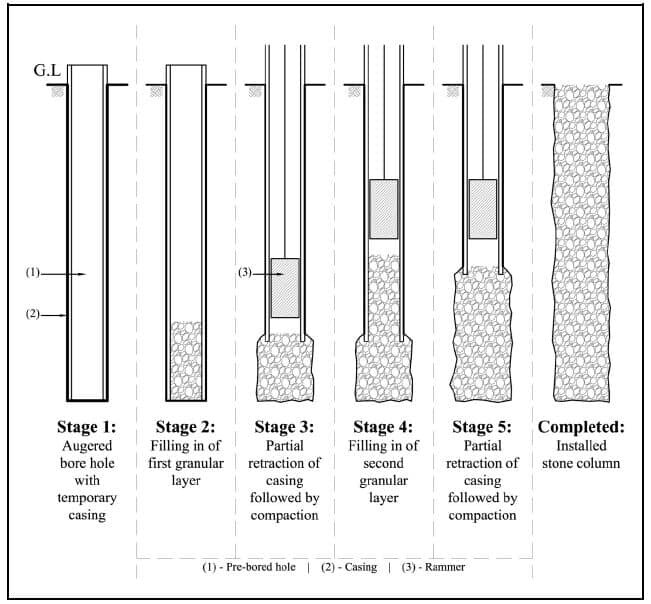
\includegraphics[height=0.5\textwidth]{stone-column-installation}
\caption{rammed-aggrgate-column-installation-2}
\label{fig:ragc_installation}
\end{figure}



 
 %%adding figure for rammed aggregate instllation
\begin{figure}[h]
\centering
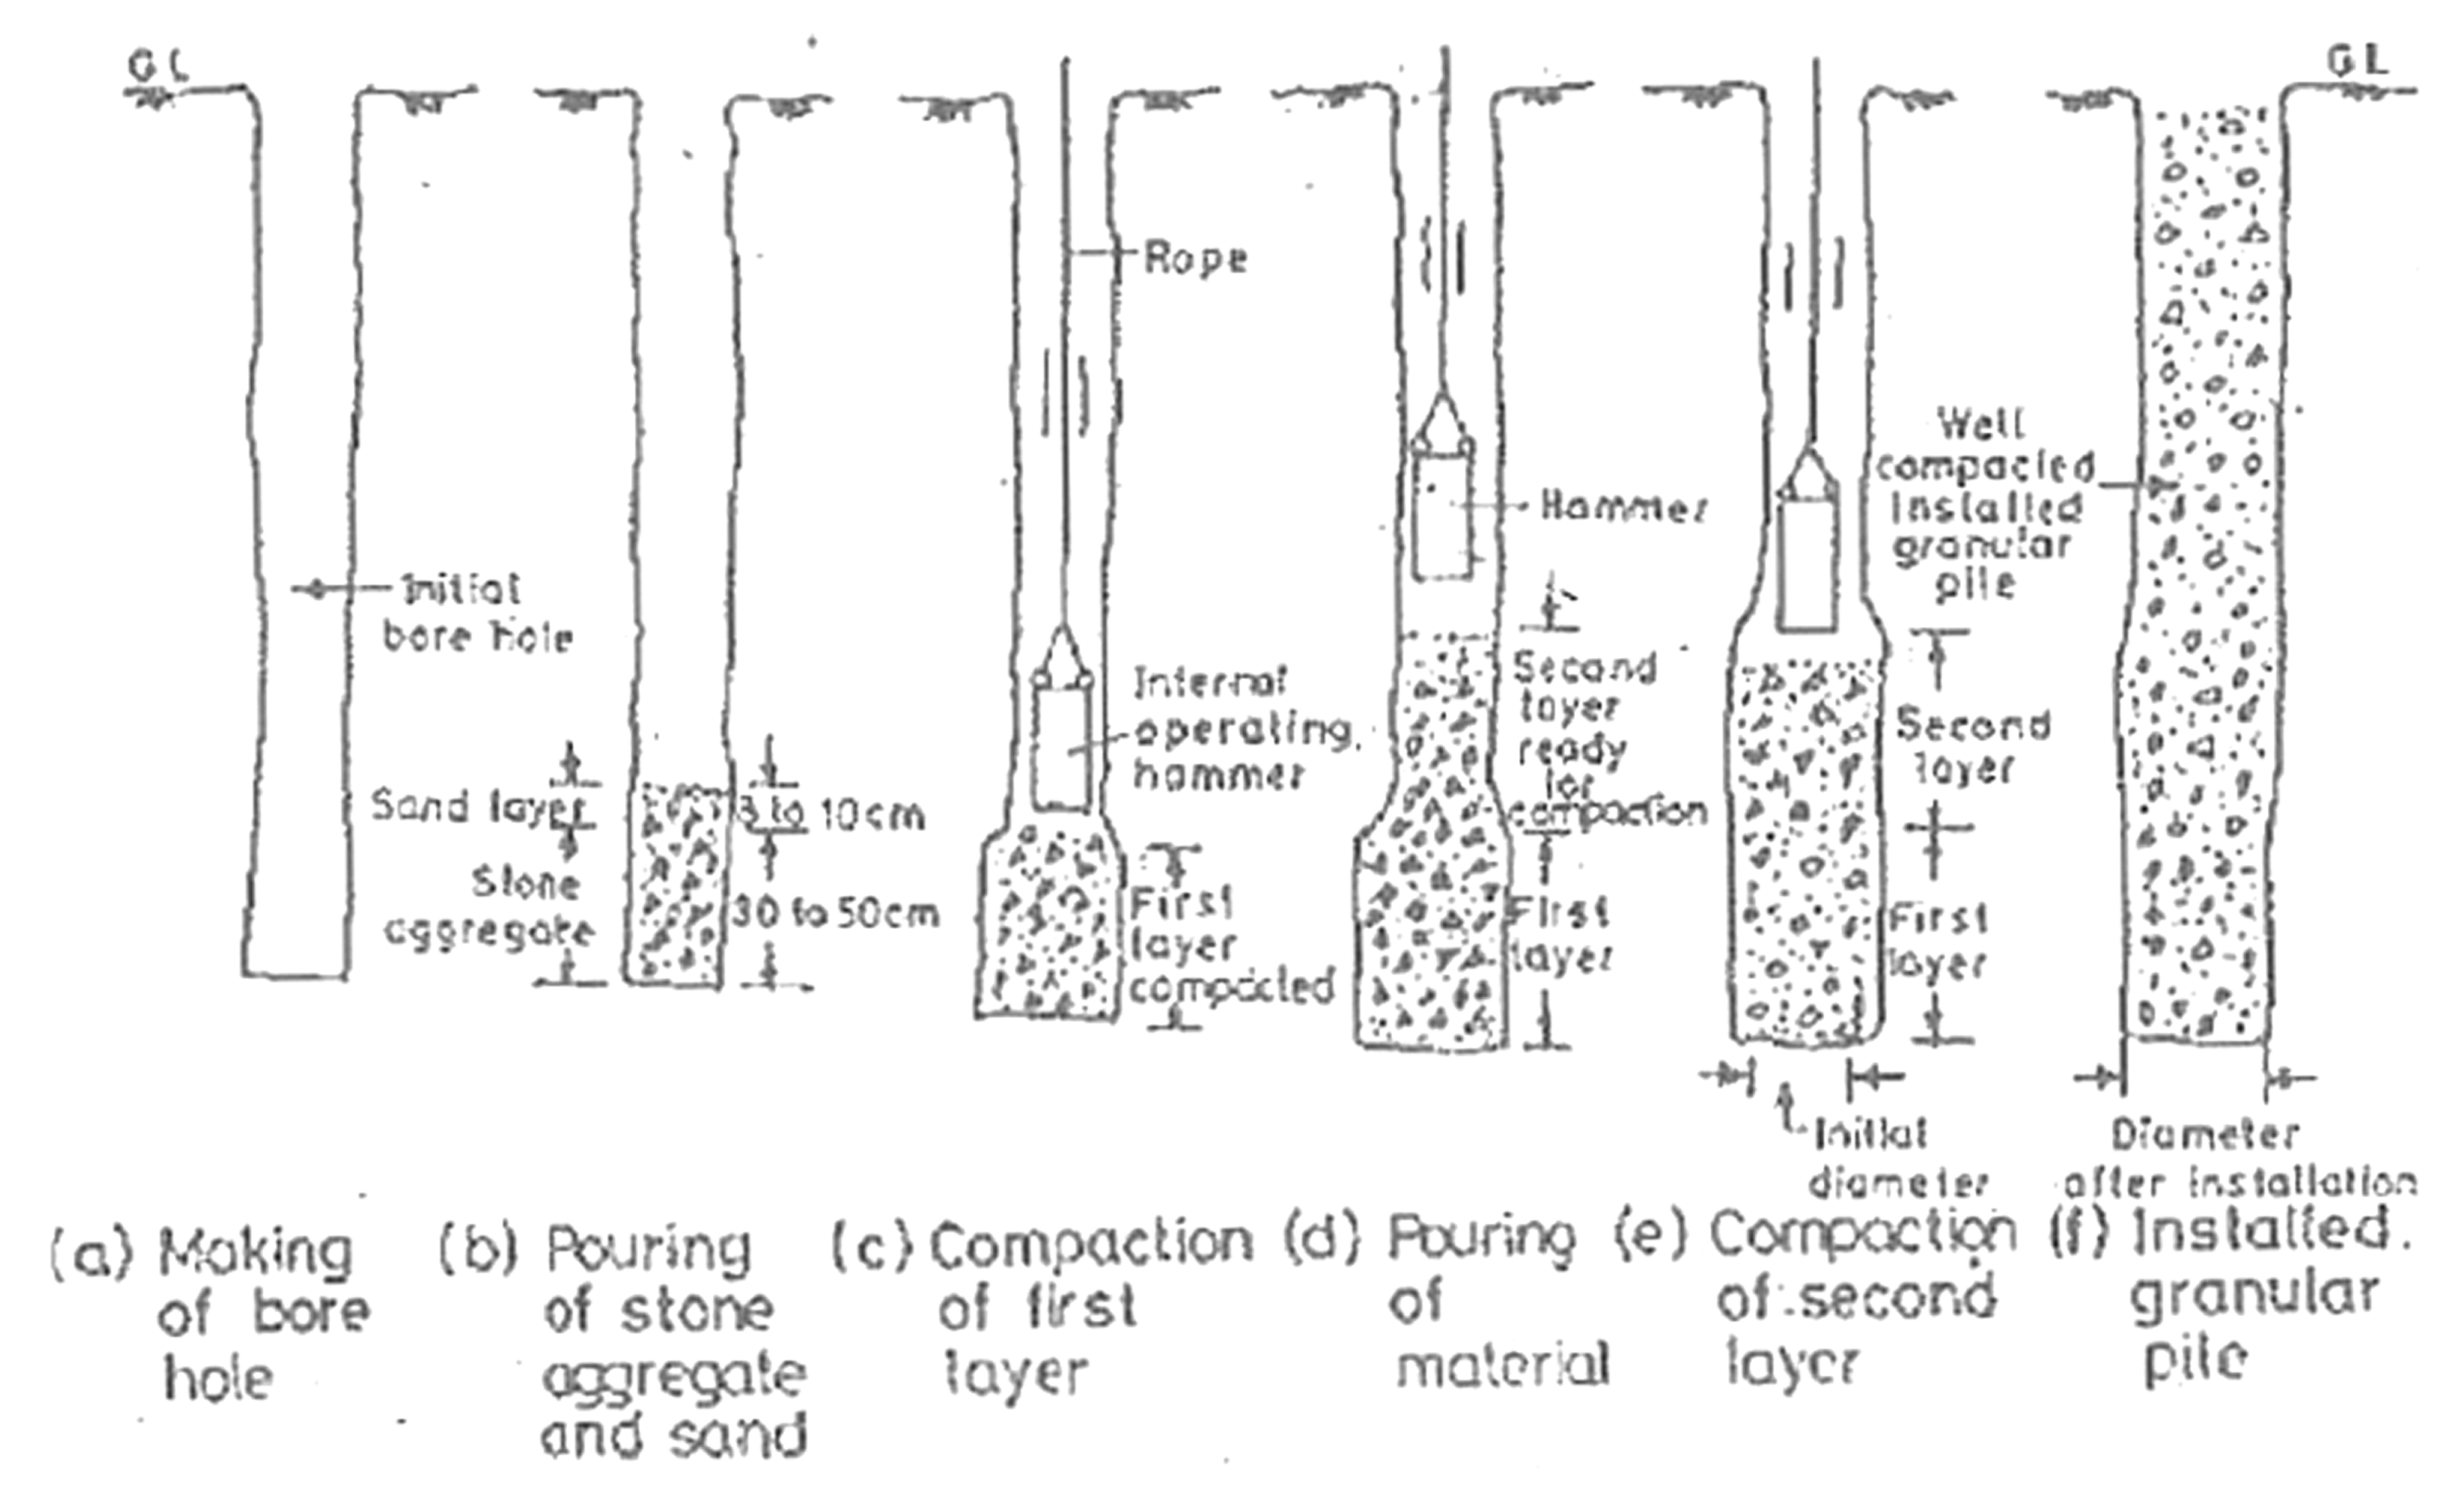
\includegraphics[height=0.5\textwidth]{Rammed_Aggret_Pile_Instalation_2}
\caption{rammed-aggrgate-column_instllation2}
\label{fig:ragc_installation2}
\end{figure}

%%end of figure

\section{Bearing Capcity Determination For Rammed Aggregate column}
The design procedure for granular columns in cohesive soils involves bearing capacity, settlement, rate of consolidation, and global slope stability. The typical procedure is as follows:
\begin{enumerate}
\item Based on undrained shear strength of cohesive soil,calculate the ultimate bearing capacity of natural soilas $5c_u$ ($c_u$ is undrained shear strength of soil).

\item Based on undrained shear strength of cohesive soil,calculate the ultimate bearing capacity of individual columns using Equation (1) 
\begin{equation}
q_{ult,c}=K^{'}K_{p}c_u
\end{equation}
\begin{equation*}
\begin{align}


K^{'}K_{p}=\text{12 for Sand Comapction Piles }\\
K^{'}K_{p}&=\text{20 for Stone Column}\\
K^{'}K_{p}&=\text{25 for Rammed Aggrgate Column} \\
\end{align}
\end{equation*}




\item Calculate the ultimate bearing capacity of the composite foundation by considering ultimate bearing capacities of natural soil and individual columns, and the area replacement ratio using Equation (2) and Equation(3).

\begin{equation}
q_{ult}=q_{ult,c}*a_{s}+q_{ult,s}*(1-a_{s})
\end{equation}

\begin{equation}
q_{ult,s}=5.14c_{u}
\end{equation}
\item determine pile dia and spacings from equation(4).

\begin{equation}
\frac{s}{d}=\sqrt{\frac{\pi}{4a_s}}
\end{equation}

\end{enumerate}


\section{SPT correlation for Clay Soil Consistency and Untrained Shear Strength }
\begin{table}[ht]
    \centering
    \begin{tabular}{|c|c|c|}
    \hline
    \textbf{SPT} & \textbf{Soil Consistency} & \textbf{$C_uKsf(KPa)$}\\
    \hline
    $<2$ & Very Soft & $0.4(20)$\\
    \hline
    $2-4$ & Soft & $0.4-0.8(20-40)$\\
    \hline
    $4-8$ & Firm & $0.8-1.5(40-75)$\\
    \hline
    $8-15$ & Stiff & $1.5-3(75-150)$\\
    \hline
    $15-30$ & Very Stiff & $3-6(150-300)$\\
    \hline
    $>30$ & Hard & \\
    \hline
    \end{tabular}
    \caption{SPT Correlation of Cohessive Soil}
    \label{tab:my_label}
\end{table}



\section{Soil Profile for 3-Vent Kjeurdangi Regulator}
it is observed from the borlog upto a depth=15.0 siol is soft-clay,below that  there is 9.2m medium clay and below that medium to dense sand.it is observed from the borlog upto a depth=15.0 siol is soft-clay,below that  there is 9.2m medium clay and below that medium to dense sand.




\begin{wrapfigure}{l}{0.9\textwidth}

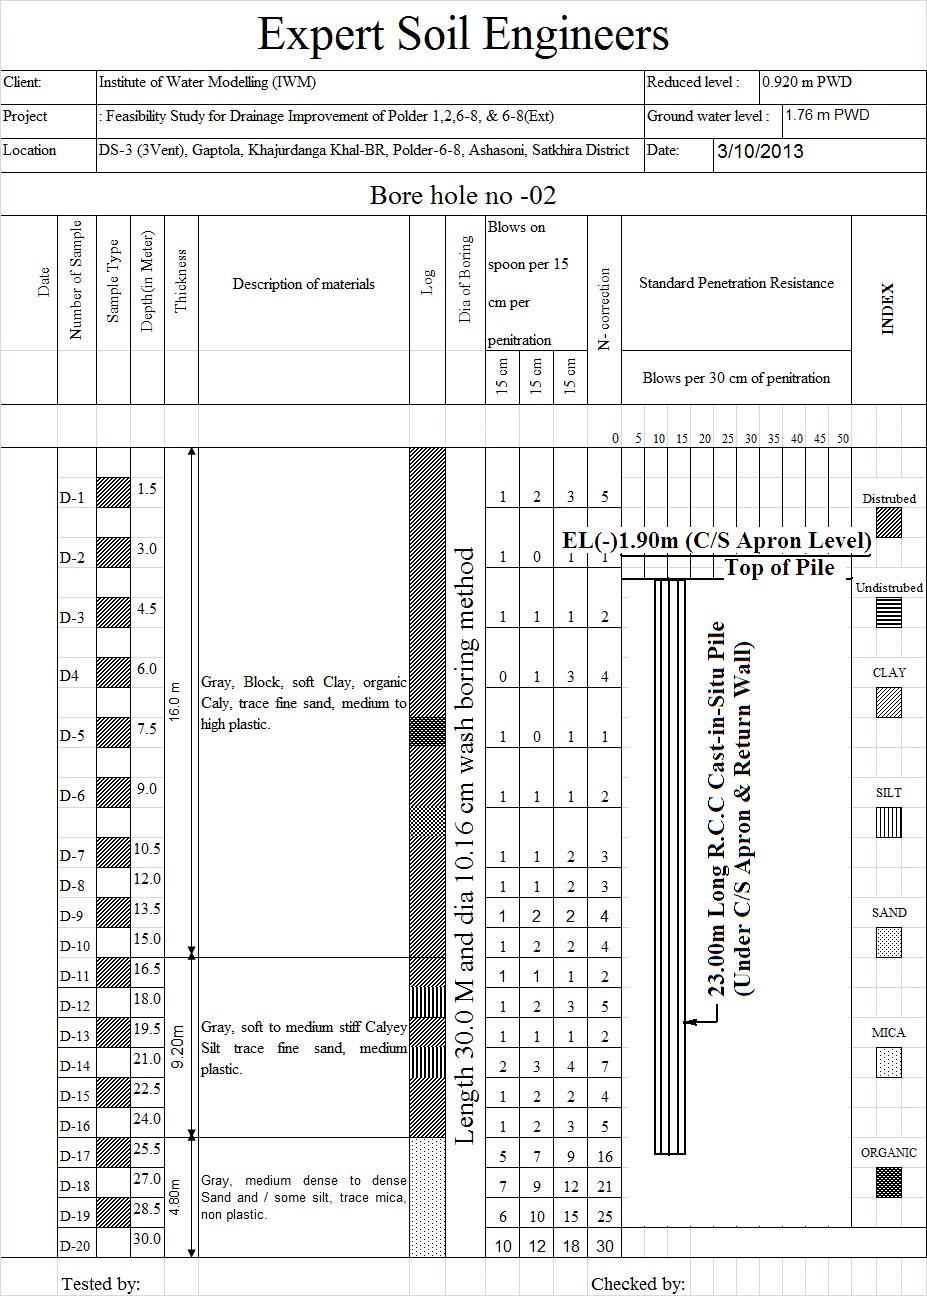
\includegraphics[height=0.9\linewidth]{borhole_2}
\caption{bore log of 3-Vent Khejurdangi Regulator}
\label{fig:bore-log}
\end{wrapfigure}
\clearpage


\section{Design Calculation}
Bearing Capacity and Settlement of Natural Ground without improvement:
\[q_{ult}=CN_CS_Cd_C+0.5{\gamma^'}{N_\gamma}{d_\gamma}+{\sigma_D^'}{N_q}{S_q}{d_q}\]\\
\begin{align*}
   \sigma{_D^'} &=(EGL-Foundation Level)*\gamma_{Sub}\\
  & =(1.5-(-)3.35)*\gamma_{Sub}\\
  & =4.85*(15-9.81)\\
  & =4.85*5.19\\
  & =25.2
\end{align*}
Assumed Values\\
$N_\gamma=0, C=5.14, S_C=d_C=1.2, N_q=S_q=d_q=1$

\begin{align*}
\ q_{ult} &=CN_CS_Cd_C+0.5{\gamma^'}{N_\gamma}{d_\gamma}+{\sigma_D^'}{N_q}{S_q}{d_q}\\
  & =37.5*5.14*1.2*1.2+0.5*0*(15-9.81)*1*1+25.2*1*1*1\\
  & =302.76 KPa\\
\end{align*}
\begin{align*}
\ q_{ult,s} &={k^'}{k_p}{C_u}\\\
  & =25*37.5\\
  & =937.5KPa\\
\end{align*}
\begin{align*}
\ q_{ult,req} &=f_s*{Foundation Pressure}\\\
  & =3*120\\
  & =360 KPa\\
\end{align*}
\begin{align*}
\ q_{ult,req} &=q_{ult,c}*a_s+{(1-a_s)}*q_{ult,s}\\\
\ 360 &=937*a_s+{(1-a_s)}*302\\\
\ 360 &=937*a_s-302*a_s+302\\\
\ 360 &=635*a_s+302\\\
\ 635*a_s &=360-302\\\
\ a_s &=\frac{58}{302}\\\
\ a_s &=0.091\\\
\end{align*}
\begin{align*}
\ \frac{s}{d} &=\sqrt\frac{\pi}{4a_s}\\\
  & =\sqrt\frac{3.14}{4*0.091}\\\
  & =2.94\\use,  2.5\\
\end{align*}
 Use 10m Rammed Aggregate Pile with s/d ratio 2.5 and 0.60m Pile dia
 
\section{Unit Cost Calculation} 
Khoa Filter:
Code: 40-520-20(40mm to 20mm)-4900.41TK\\
Code: 40-520-30(20mm to 5mm)-5401.45TK\\
Material Cost=5150\\
Total cost including Installation Cost and VAT-Tax= 5350*1.33*1.2=8540

unit cost=$m^3$=164440 BDT=0.0854 lakh BDT

\section{Foundation Cost for Regulator}
Regulator Foot print Ares=$635 m^{2}$\\
depth of improvement=10 m\\
Total soil volume=$6350 m^{3}$\\
Total Pile Volume=0.125*6350=$$790 m^{3}$\\
Total cost=0.0854*790=68 Lakh BDT\\

 
\end{document}

